\section{Lavoro di una forza}
Il lavoro di una forza è la quantità di energia scambiata tra due sistemi, quando avviene uno spostamento per mezzo di una forza. Matematicamente è definito come l'integrale della forza lungo una curva, ovvero il percorso lungo cui si sposta il corpo.
\begin{equation}
\boxed{W = \int_\gamma d\vec s \cdot \vec F}
\end{equation}
Ne segue che la forza è sempre ortogonale allo spostamento, questa non compierà lavoro sul corpo. Se pensiamo ad $\vec F$ come una risultante delle forze otterremo che:

\begin{equation}
W =  \int_\gamma d\vec s \cdot \sum_{k=1}^n\vec F_k = \sum_{k=1}^n \int_\gamma d\vec s \cdot \vec F_k = \sum_{k=1}^n W_k
\end{equation}
Il lavoro totale può essere visto come la somma dei lavori delle singole forze che costituiscono $\vec F$.
Se il lavoro è positivo, allora di dice lavoro motore, mentre se è negativo si dice lavoro resistente.
Il lavoro essendo un'energia è misurato nel S.I. con il $(J)$ Joule. Un Joule è definito come l'energia scambiata da una forza di un Newton, per compiere uno spostamento di un metro lungo la sua stessa direzione: $1J = 1N\cdot 1 m$. 

\subsection{Potenza}
La potenza esprime la velocità con cui viene trasferita una particolare forma di energia. Adesso parleremo di potenza meccanica, definita come la derivata rispetto al tempo del lavoro, ed è misurata in Watt $(W)$. Una potenza di un Watt trasferisce un Joule in un secondo.
\begin{equation}
\boxed{P=\frac{dW}{dt}}
\end{equation}

\subsection{Lavoro come variazione di energia cinetica}
Scriviamo il lavoro infinitesimo per una forza generica data da $\vec F = m\vec a$.
\begin{equation}
dW = \vec F\cdot d\vec s = ma_tds = m\dot v ds = mv dv 
\end{equation}
Integrando otterremo che il lavoro per spostare il corpo dal punto $A$ al punto $B$ sarà:
\begin{equation}
W = \int_{v_A}^{v_B}mvdv = \frac12mv_B^2- \frac12mv_A^2
\end{equation}
Quindi definendo l'energia cinetica, l'energia associata al movimento di un corpo, come $K = \frac12 mv^2=\frac{p^2}{2m}$, otteniamo che:
\begin{equation}
W = K_B - K_A = \Delta K
\end{equation}

\subsection{Lavoro della forza gravitazionale}
Prendiamo il caso in cui la forza peso faccia spostare un corpo di massa $m$ da un punto $A$ ad un punto $B$, a quota più bassa di $A$. Supponiamo che il corpo segua un percorso a piacere, purché vada da $A$ a $B$. quindi prendo un asse verticale $z$ diretto verso l'alto, otterremo che:
\begin{figure}[htbp]
\begin{center}
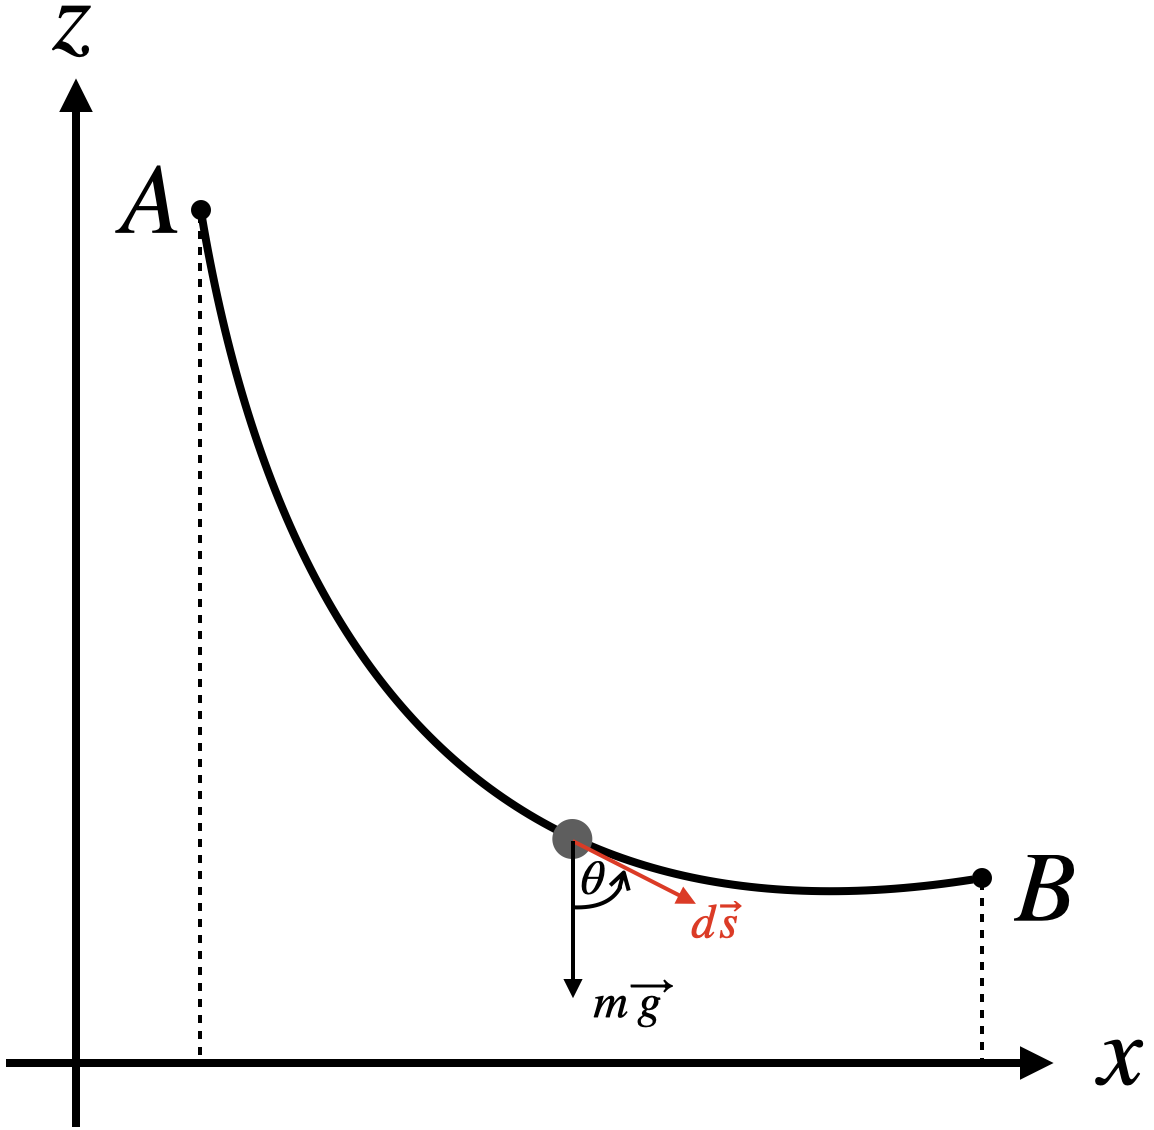
\includegraphics[width=10cm]{images/lavorog.png}
\caption{Rappresentazione del lavoro infinitesimo lungo un tratto elementare di curva $d\vec s$ del forza gravitazionale $\vec F_p = m\vec g$.}
\label{default}
\end{center}
\end{figure}

\begin{equation}
W = \int_A^Bd\vec s \cdot\vec F_p = -mg\int_A^Bds\cos\theta = -mg\int_A^Bdz = -mg\sx z_B-z_A\dx
\end{equation}

Ovvero definendo l'energia potenziale gravitazionale come $U = mgz$, abbiamo che il lavoro è meno la variazione di energia potenziale:

\begin{equation}
W = U_A-U_B = -\Delta U
\end{equation}

imponendo uguali le equazioni $(2.48)$ e $(2.50)$ otteniamo il principio di conservazione dell'energia meccanica $E = K + U$.
\begin{equation}
\Delta K = -\Delta U\seg K_B-K_A = U_A -U_B\seg K_A+U_A = K_B+U_B\seg \boxed{E_A = E_B}
\end{equation}

\subsection{Lavoro della forza elastica}

Calcoliamo il lavoro di una forza elastica diretta lungo $x$: $\vec F_e = -kx\hat\imath$.
\begin{equation}
W = -k\int_A^Bdx x = \frac12 kx_A^2-\frac12 kx^2_B\quad\quad U_e = \frac12 kx^2\seg W = -\Delta U_e
\end{equation}

\subsection{Lavoro della forza d'attrito radente}
La forza d'attrito, essendo sempre diretta in verso opposto alla velocità produce un lavoro negativo, ovvero sempre resistente. L'integrale sulla curva dipende dal percorso scelto, al contrario delle forze conservative, e quindi in un percorso chiuso il lavoro d'attrito sarà diverso da zero.

\begin{equation}
\vec F_a = -\mu_d N \hat u_v\seg W_a = -\mu_d\int_A^BdsN = -\mu_dN\Delta s
\end{equation}

\subsection{Lavoro di forze conservative e non conservative}
Come abbiamo visto, il lavoro di una forza conservativa, che ammette un'energia potenziale, non dipende dal percorso su cui si integra, ne segue che se scegliamo un percorso chiuso l'integrale sulla curva chiusa sarà sempre nullo. \\Quindi se $\vec F$ è una forza conservativa ne segue che:

\begin{equation}
\boxed{\oint_\gamma d\vec s \cdot F = 0}
\end{equation}

Dunque in questi casi che l'energia meccanica si conserva, quindi l'energia meccanica nello stato iniziale è uguale all'energia meccanica nello stato finale:
\begin{equation}
\boxed{E_i = E_f}
\end{equation}
Mentre nel caso in cui sono presenti forze non conservative, il lavoro delle forze non conservative non è nullo ed è pari alla variazione di energia meccanica. E dato che durante il processo si dissipa energia:
\begin{equation}
\boxed{W_{NC} = \Delta E = E_f- E_i < 0}
\end{equation}

Se prendiamo una generica forza $\vec F_{\sx x,y,z\dx} = \sx F_x,F_y,F_z\dx$, se supponiamo che essa sia conservativa possiamo scrivere che:
\begin{equation}
\int_A^Bd\vec s\cdot \vec F = \int F_xdx+F_ydy+F_zdz
\end{equation}
Ora se ammettiamo l'esistenza di un'energia potenziale, tale per cui la forza è il suo gradiente cambiato di segno:
\begin{equation}
\vec F_{\sx x,y,z\dx} = -\vec\nabla U_{\sx x,y,z\dx} = -\sx\frac{\partial U}{\partial x},\frac{\partial U}{\partial y},\frac{\partial U}{\partial z}\dx
\end{equation}
Trovandoci in questa situazione avremo che:
\begin{equation}
\int_A^B F_xdx+F_ydy+F_zdz = -\int\vec \nabla U\cdot d\vec x = -\int dU = -\sss U_{(B)}-U_{(A)}\ddd = -\Delta U
\end{equation}
Come possiamo notare i risultati ottenuti nelle equazioni $(2.50)$ e $(2.52)$, sono in realtà molto più generali e, data una forza esprimibile come il gradiente di un'energia potenziale (cambiato di segno), si avrà che il lavoro da un punto $A$ a un punto $B$ seguendo una qualsiasi curva, sarà pari a meno la variazione di energia potenziale. Di conseguenza una volta appreso queso fatto, possiamo capire facilmente il perchè dell'equazione $(2.54)$. Se si sceglie una curva chiusa, punto $A$ coincide con il punto $B$ dunque dato che l'energia potenziale iniziale e finale sono uguali, il lavoro è nullo.

\section{Momento angolare}
Il momento angolare è una grandezza molto importante in fisica, esso è definito come il prodotto vettoriale tra il raggio vettore ed il vettore impulso. È analogo alla quantità di moto in quanto, infatti esprime un concetto di resistenza non al cambio di velocità lineare come nel caso dell'impulso, ma al cambiamento dello stato di rotazione di un corpo.
Infatti se un corpo ha un momento angolare costante nel tempo, allora si muove di moto circolare uniforme. Mentre se il momento angolare varia nel tempo, esisterà un'accelerazione angolare.

\begin{equation}
\boxed{\vec L = \vec r \times \vec p = \vec r \times m\vec v}
\end{equation}
È importante ricordare che il momento angolare è uno pseudo-vettore in quanto ha una forma diversa in base al polo rispetto al quale viene calcolato. Ad esempio se trasliamo l'origine degli assi $O$ in $O'$, come mostrato in figura $(2.11)$, otterremo che:
\begin{equation}
\vec L = \vec r \times \vec p\quad \quad \vec L' = \vec r '\times\vec p = \sx\vec r + \vec t\dx\times \vec p = \vec r \times \vec p + \vec t\times\vec p = \vec L + \vec t\times\vec p
\end{equation}
Quindi traslando il polo otterremo una variazione del momento angolare che è la seguente:
\begin{equation}
\boxed{\vec L'-\vec L = \vec t\times\vec p}
\end{equation}
 
 \begin{figure}[htbp]
\begin{center}
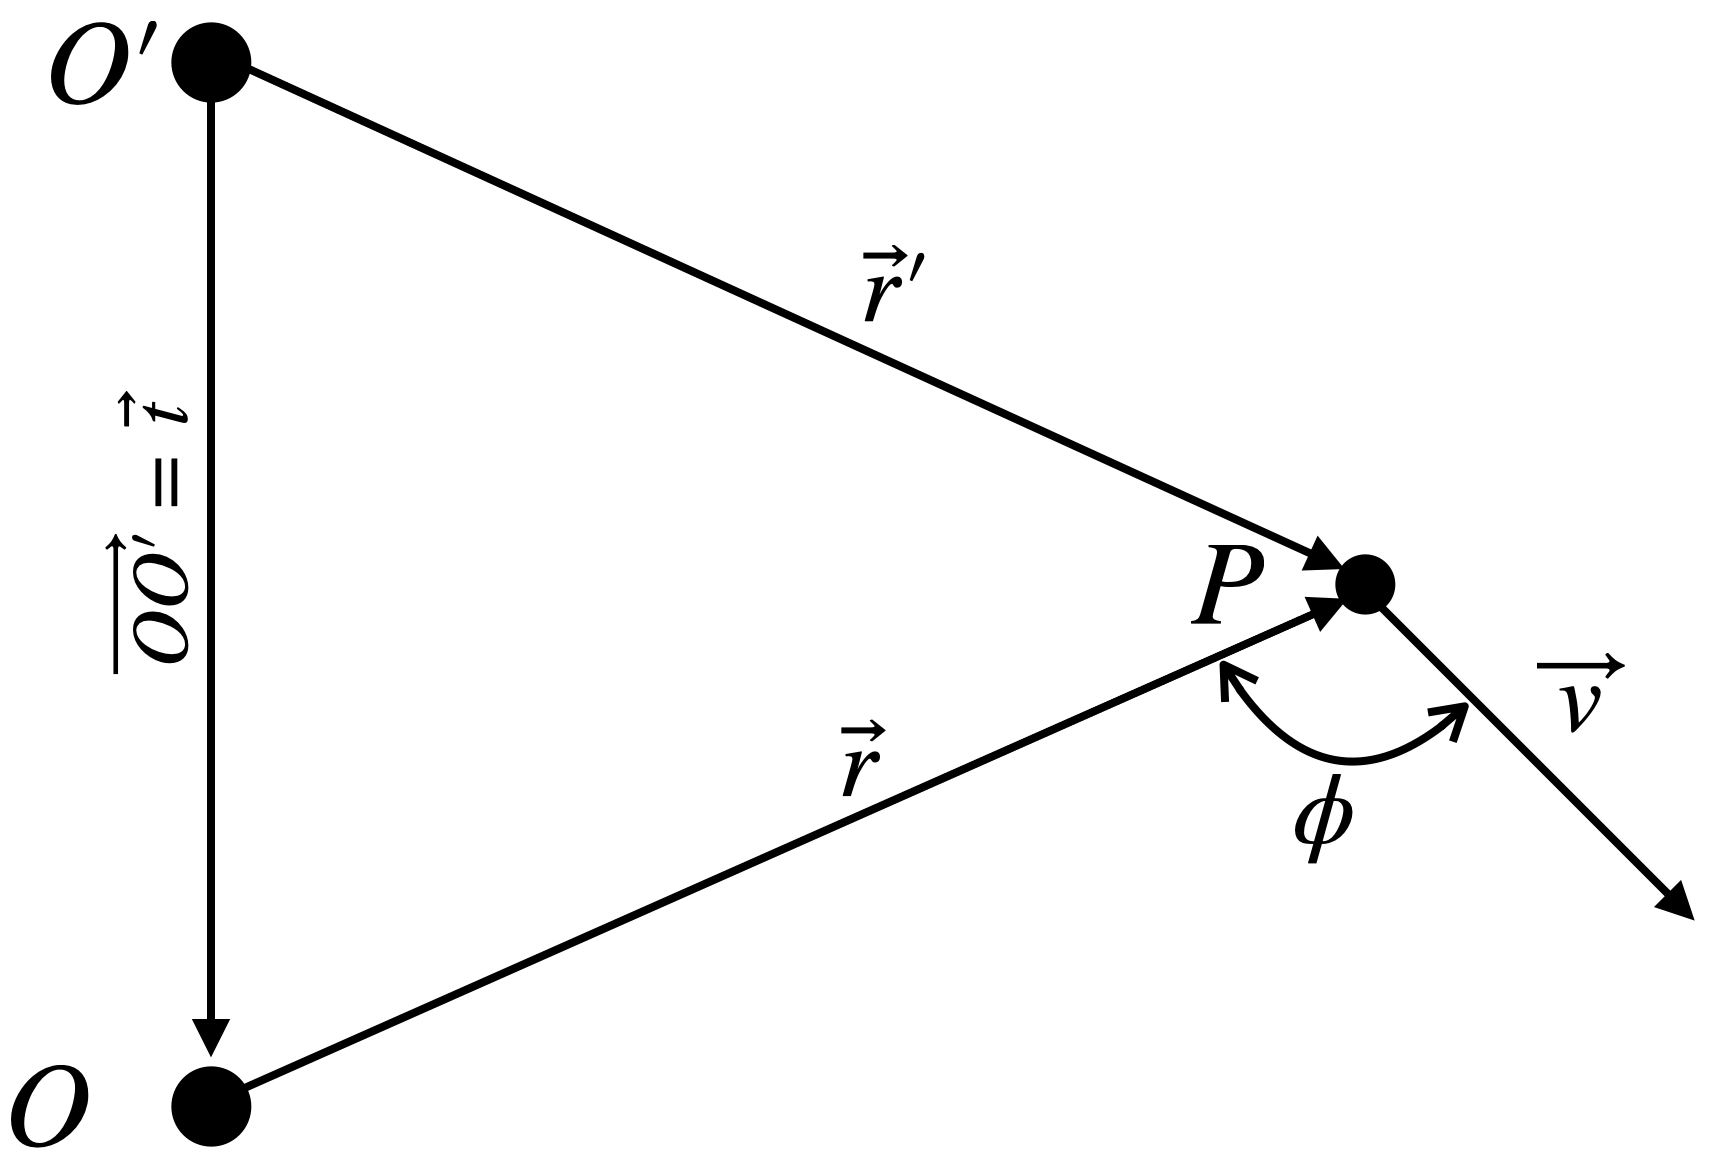
\includegraphics[width=10cm]{images/momang1.png}
\caption{Schema dei vettori $\vec r$, $\vec r'$, $\vec v$ e $\vec t$, utilizzati per il calcolo del momento angolare rispetto ai poli $O$ ed $O'$.}
\label{default}
\end{center}
\end{figure}
In coordinate polari possiamo scrivere la velocità come somma della sua componente radiale e quella trasversa, ne segue che dato che la componente radiale è ortogonale al raggio vettore, essa non da contributo al momento angolare.

\begin{equation}
\vec L = \vec r \times m\sx \vec v_r+\vec v_\phi\dx = \vec r \times m\vec v_\phi
\end{equation}

Quindi dato che $\vec v_\phi = r\frac{d\phi}{dt}$ possiamo scrivere il modulo del momento angolare di un punto materiale nel seguente modo:

\begin{equation}
\boxed{L = mr^2\frac{d\phi}{dt} = I\omega}
\end{equation}

Dove abbiamo chiamato $I$ il momento d'inerzia. Il momento d'inerzia è un analogo del termine di massa che compare nella definizione di impulso, quindi come la massa esprime un concetto di resistenza alla variazione dello stato di moto, il momento d'inerzia rappresenta lo stesso concetto, ma per moti rotatori. Da notare dunque l'analogia in formule: $\vec p$ con $\vec L$, $m$ con $I$ e $\vec v$ con $\vec \omega$.
\begin{equation}
\vec p = m\vec v \quad\quad \quad \vec L = I\vec     \omega
\end{equation} 

In questo caso il momento d'inerzia di un punto che ruota su una circonferenza di raggio $r$ è pari ad $I = mr^2$. Vedremo poi in seguito, nel capitolo sui corpo rigidi, come in realtà questo momento d'inerzia per corpo estesi è una matrice, dunque in generale potremmo incontrare casi in cui il momento angolare non è parallelo alla velocità angolare.             

\subsection{Momento di una forza}
In analogia con il momento angolare, il momento di una forza è definito dal prodotto vettoriale tra il raggio vettore e la forza.

\begin{equation}
\boxed{\vec M = \vec r \times \vec F}
\end{equation}

Partendo dalla definizione di momento angolare, si può effettuare la derivata rispetto al tempo ottenendo infine la relazione che lega momento angolare e momento delle forze.

\begin{equation}
\vec L = \vec r \times \vec p \seg \frac{d\vec L}{dt} = \cancel{\vec v\times\vec p} + \vec r \times \frac{d\vec p}{dt} \seg \boxed{\vec M = \frac{d\vec L}{dt}}
\end{equation}

\section{Teorema dell'impulso angolare}
Analogamente a quanto fatto per il teorema dell'impulso, iniziamo integrando l'equazione $(2.67)$.

\begin{equation}
\vec M = \frac{d\vec L}{dt} \seg \int_0^\tau dt\frac{d\vec L}{dt} = \int_0^\tau dt \vec M \seg \Delta \vec L =\int_0^\tau dt \vec M 
\end{equation}
\begin{equation}
\vec{M_m} = \frac1\tau\int_0^\tau dt \vec M = \frac{\Delta \vec L}{\tau}
\end{equation}














